\documentclass{article}
\usepackage{graphicx}
\usepackage{hyperref}
\begin{document}
\title{Multicast Routing in Linux}
\author{Ang Way Chuang \\
\small{\href{mailto:wcang79@gmail.com}{wcang79@gmail.com}}}
\date{\today}
\maketitle
\section{Foreword}
This is part of an ongoing effort to understand how multicast forwarding works
and implementation of multicast routing within a routing daemon on Linux (UNIX)
system. Those who want to look for guide to write multicast application should
look elsewhere. As my understanding on multicast routing is quite limited,
errors are to be expected and the document will remain incomplete and
disorganized until I have a better understanding on the subject. I would like to
thank Achmad Basuki for his encouragement and his eargerness to share his
knowledge. You're my routing god.

There are a lot of online references on PIM multicast routing, but there is
hardly none that discuss how it is implemented in Linux. This document tries to
address that gap. Each section will try to address the WHY first before diving
into the finer aspect. This document refers to the implementation of Linux
kernel version 3, but the discussion should apply to older and newer kernels
that implements multicast routing. Due to time limit, this document shall limit
itself to IPv6.

\section{Multicast Forwarding}
\begin{figure}[!h]
  \begin{center}
    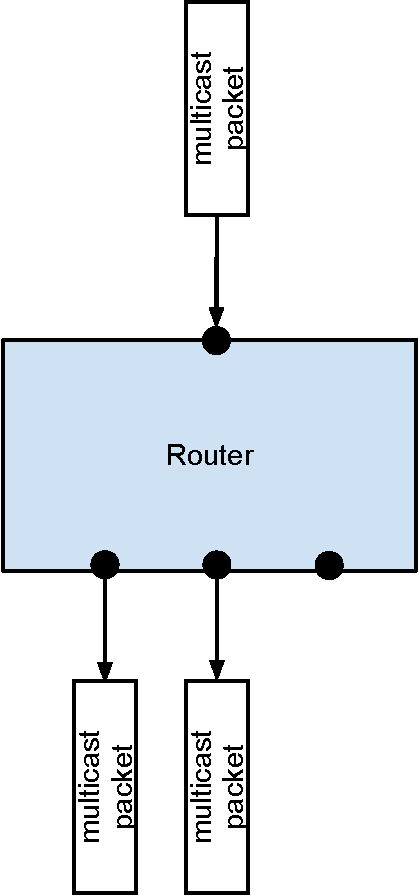
\includegraphics[width=0.3\textwidth]{mcast-forward}
    \caption{Router duplicates and send out multicast packet to the
    outgoing interfaces that have active listeners of multicast group}
    \label{fig:mcast-forward}
  \end{center}
\end{figure}

As shown in Figure \ref{fig:mcast-forward}, unlike unicast forwarding, when a
multicast packet is received by a router, the packet may be forwarded to
multiple outgoing interfaces. While, it is the job of the kernel to duplicate
the packet and forward the multicast packet to all the relevant outgoing
interfaces, the kernel doesn't know which interfaces to forward the multicast
packet. 

Routing daemon running PIM protocol will learn about the active listeners of the
multicast stream and therefore which outgoing interfaces where the multicast
packet should be forwarded. Therefore, it is the job of routing daemon to
instruct the kernel on this matter by adding multicast forwarding cache (MFC).

MFC basically consists of the following tuple:
\begin{itemize}
  \item source address - source (S) address of multicast packet
  \item group address - group (G) address of multicast packet
  \item incoming interface - the network interface where the multicast packet
  belonging to the (S,G) should be received. TODO: need to know why this need to
  be specified as it is assumed that the kernel should have the required
  knowledge to the RPF checking and therefore it can derive this information
  using RIB. Is this there due to legacy of KAME implementation? Is there any
  valid reason why this need to specified by user space routing daemon?
  \item list of outgoing interfaces - the network interfaces where the multicast
  packet should be forwarded 
\end{itemize}

User space routing daemon can manipulate MFC using \texttt{mf6cctl\{\}}
(\texttt{<linux/mroute6.h>}). Within the kernel, MFC entry is represented by
\texttt{mfc6\_cache\{\}} (\texttt{include/linux/mroute6.h}).

\subsection{Interaction}
Diagram
\begin{figure}[!h]
  \begin{center}
    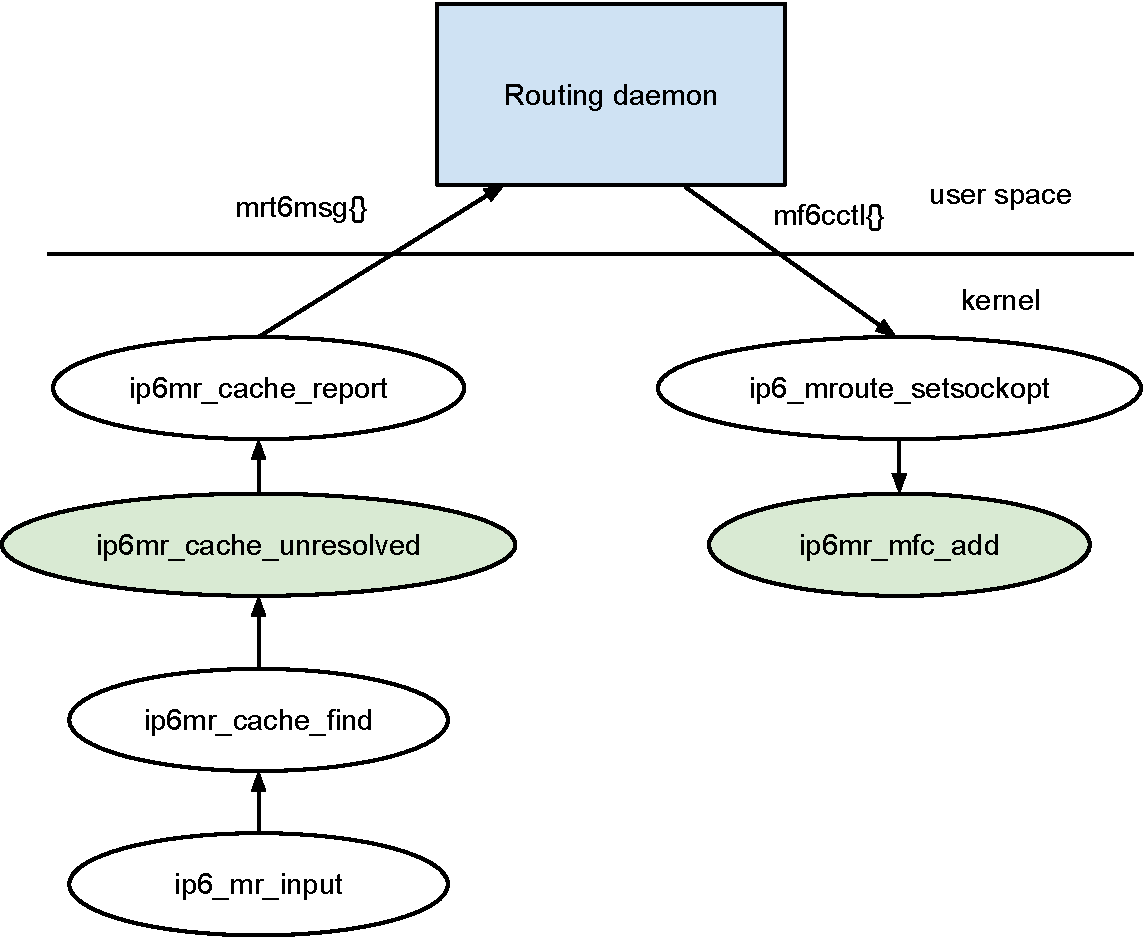
\includegraphics[width=0.75\textwidth]{mcast-unresolved}
    \caption{Interaction between kernel and user space routing daemon when MFC
    is not available during multicast forwarding}
    \label{fig:mcast-unresolved}
  \end{center}
\end{figure}

\begin{figure}[!h]
  \begin{center}
    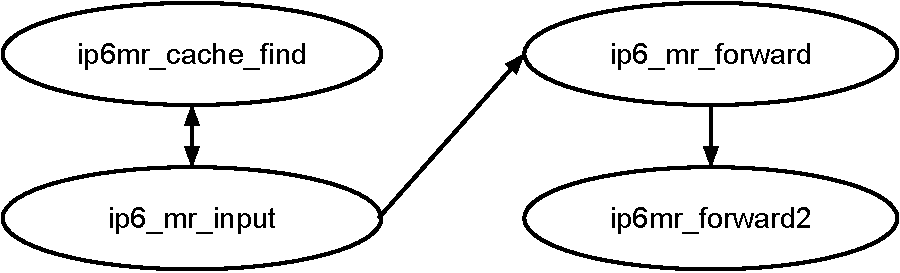
\includegraphics[width=0.6\textwidth]{mcast-mfc}
    \caption{Multicast forwarding when MFC is available}
    \label{fig:mcast-mfc}
  \end{center}
\end{figure}


Not sure why there is a need to store unresolved multicast packet as I presume
that routing daemon should be proactive in setting up multicast routing cache
whenever it learns of a new PIM JOIN. Why should it wait for kernel to inform
it of the new route? Is it because of measure to save memory until it is really
needed?


\section{References}
IPv6 Advanced Protocol Implementations

RFC 4601

http://manpages.ubuntu.com/manpages/hardy/man4/multicast.4.html

http://manpages.ubuntu.com/manpages/hardy/man4/pim.4.html

\end{document}
